\documentclass[letterpaper]{article}
\usepackage[margin=1in]{geometry}
\usepackage[utf8]{inputenc}
\usepackage{textcomp}
\usepackage{amssymb}
\usepackage{natbib}
\usepackage{graphicx}
\usepackage{gensymb}
\usepackage{amsthm, amsmath, mathtools}
\usepackage[dvipsnames]{xcolor}
\usepackage{enumerate}
\usepackage{mdframed}
\usepackage[most]{tcolorbox}
\usepackage{csquotes}
% https://tex.stackexchange.com/questions/13506/how-to-continue-the-framed-text-box-on-multiple-pages

\tcbuselibrary{theorems}

\newcommand{\R}{\mathbb{R}}
\newcommand{\Z}{\mathbb{Z}}
\newcommand{\N}{\mathbb{N}}
\newcommand{\Q}{\mathbb{Q}}
\newcommand{\C}{\mathbb{C}}
\newcommand{\code}[1]{\texttt{#1}}
\newcommand{\mdiamond}{$\diamondsuit$}
\newcommand{\PowerSet}{\mathcal{P}}
\newcommand{\Mod}[1]{\ (\mathrm{mod}\ #1)}
\DeclareMathOperator{\lcm}{lcm}

%\newtheorem*{theorem}{Theorem}
%\newtheorem*{definition}{Definition}
%\newtheorem*{corollary}{Corollary}
%\newtheorem*{lemma}{Lemma}
\newtheorem*{proposition}{Proposition}


\newtcbtheorem[number within=section]{theorem}{Theorem}
{colback=green!5,colframe=green!35!black,fonttitle=\bfseries}{th}

\newtcbtheorem[number within=section]{definition}{Definition}
{colback=blue!5,colframe=blue!35!black,fonttitle=\bfseries}{def}

\newtcbtheorem[number within=section]{corollary}{Corollary}
{colback=yellow!5,colframe=yellow!35!black,fonttitle=\bfseries}{cor}

\newtcbtheorem[number within=section]{lemma}{Lemma}
{colback=red!5,colframe=red!35!black,fonttitle=\bfseries}{lem}

\newtcbtheorem[number within=section]{example}{Example}
{colback=white!5,colframe=white!35!black,fonttitle=\bfseries}{def}

\newtcbtheorem[number within=section]{note}{Important Note}{
        enhanced,
        sharp corners,
        attach boxed title to top left={
            xshift=-1mm,
            yshift=-5mm,
            yshifttext=-1mm
        },
        top=1.5em,
        colback=white,
        colframe=black,
        fonttitle=\bfseries,
        boxed title style={
            sharp corners,
            size=small,
            colback=red!75!black,
            colframe=red!75!black,
        } 
    }{impnote}
\usepackage[utf8]{inputenc}
\usepackage[english]{babel}
\usepackage{fancyhdr}
\usepackage[hidelinks]{hyperref}

\pagestyle{fancy}
\fancyhf{}
\rhead{CSE 131}
\chead{Wednesday, April 12, 2023}
\lhead{Lecture 5}
\rfoot{\thepage}

\setlength{\parindent}{0pt}

\begin{document}
\section{Local Variables}
In this lecture, we want to add support for local variables through \code{let} expressions. 

\begin{mdframed}
    (Exercise.) Consider the following code.
    \begin{verbatim}
        (let (x 10)
            (let (y 10)
                (+ x y)))\end{verbatim}
    Using code discussed in the previous section, along with some intuition, what assembly do you think should be produced?

    \begin{mdframed}
    \end{mdframed}
    The assembly that could possibly be produced is as follows:
    \begin{center}
        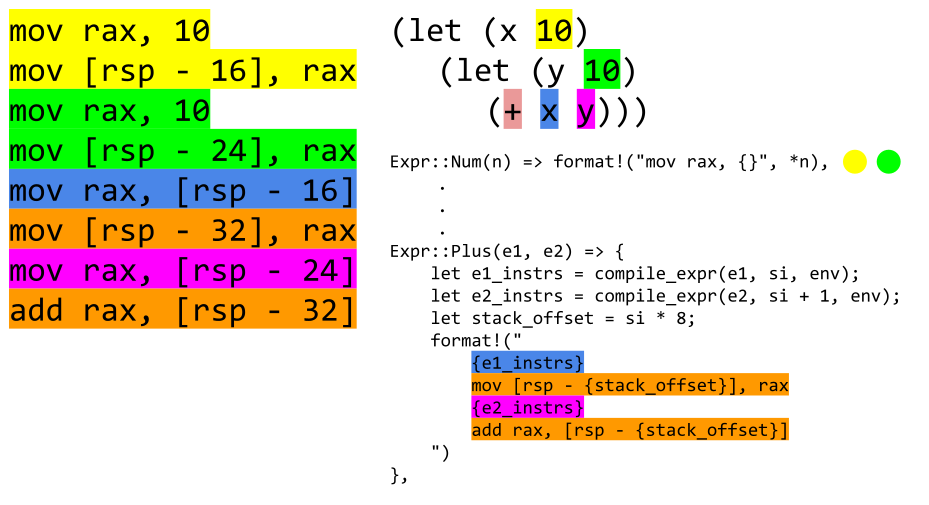
\includegraphics[scale=0.45]{../assets/let_intro_asm.png}
    \end{center}
    
    At a high level, in terms of variable declaration, 
    \begin{itemize}
        \item We defined a local variable \code{x} with value \code{10}. So, it would make sense to store the value somewhere (e.g., at location \code{rsp - 16} in the stack). This corresponds to the first two lines of assembly, which are highlighted yellow.
        \item In the body of the first \code{let}-expression, we defined a local variable \code{y} with value \code{10}. So, again, it would make sense to store this value somewhere (e.g., at location \code{rsp - 24} in the stack, since we wouldn't want to overwrite the value at \code{rsp - 16}). This corresponds to the second two lines of assembly, highlighted orange. 
    \end{itemize}
    Next, we're performing the addition. Note that we're working with the expression \code{(+ x y)}. The assembly generated by the addition is found under the \code{Expr::Plus} branch.   
    \begin{itemize}
        \item It would make sense to put the value corresponding to \code{x} into our register where we're storing the answer, \code{rax}. Since the value corresponding to \code{x} is stored in the stack (at location \code{rsp - 16}), we need to \emph{move} the value over to \code{rax}. This corresponds to the fifth line in the assembly (highlighted blue). In this sense, we can assume that \code{e1\_instrs} returns just that line: \code{mov rax, [rsp - 16]}.
        \item Next, according to how we defined the instructions for addition, we need to move the value stored in \code{rax} to the stack memory, \code{[rsp - 32]}. This corresponds to the sixth line in the assembly (highlighted orange). Note that \code{32} is picked since we don't want to write this value to \code{rsp - 24} (this would overwrite \code{y}'s value.)
        \item Similarly, for variable \code{y}, we need to store its value into the register \code{rax}. Remember that \code{y}'s value is stored in the stack at location \code{rsp - 24}. So, we can move the value from this location to \code{rax}. This corresponds to the seventh line in the assembly (highlighted pink).
        \item Finally, from the last line in the \code{Expr::Plus} branch, we need to add the value stored at \code{rsp - 32} to \code{rax}. Recall that \code{[rsp - 32]} has \code{x}'s value (since we moved \code{x}'s value to \code{[rsp - 32]} from the previous two steps). This corresponds to the last line in the assembly (highlighted orange).
    \end{itemize}
    This gives us the desired result in \code{rax}.
\end{mdframed}
There are several things we want to consider here.
\begin{itemize}
    \item How do we modify the grammar and our code to account for these changes?
    \item How do we store the identifiers and their stack offsets? 
\end{itemize}

\subsection{Grammar and AST}
Our expression now takes on two new forms:
\begin{itemize}
    \item A \code{let} expression, which takes a \emph{binding} consisting of an identifier and an associated expression, and additionally a corresponding body to be executed. 
    \item An identifier expression itself (this is how we refer to an identifier). 
\end{itemize}
Our grammar will look something like this: 
\begin{verbatim}
    (*
        expr := <number>
            | (add1 <expr>)
            | (sub1 <expr>)
            | (+ <expr> <expr>)
            | (let (<name> <expr>) <expr>)
            | <name>
    *)\end{verbatim}
The \code{Expr} \code{enum}, our AST representation, might look like 
\begin{verbatim}
    enum Expr {
        Num(i32),
        Add1(Box<Expr>),
        Sub1(Box<Expr>),
        Plus(Box<Expr>, Box<Expr>),
        Let(String, Box<Expr>, Box<Expr>),
        Id(String),
    }\end{verbatim} 
To reiterate, in \code{Let(String, Box<Expr>, Box<Expr>)}, 
\begin{itemize}
    \item The \code{String} and first \code{Box<Expr>} represents the \emph{binding}, where the \code{String} is the identifier and the first \code{Box<Expr>} is the expression. Here, we're associating the expression to the identifier. 
    \item The last \code{Box<Expr>} is the \emph{body} that follows the \code{let}-expression.
\end{itemize}

\subsection{Modifying the Parser}
We need to modify our parser to account for the two different expressions, the \code{let} expression and the identifier expression. 

\subsubsection{The \code{let}-Binding}
Remember that, in the s-expression, the \code{let}-binding will look like 
\begin{verbatim}
    (let (<name> <expr>) <expr>)
     [a]   [b]     [c]     [d]\end{verbatim}
Here, this corresponds to having a List of atoms and expressions. Namely, we have 
\begin{itemize}
    \item (a) an atom with a \code{String} value equal to \code{let} (this is how we know this is a \code{let}-binding),
    \item an \emph{expression}, represented as a \code{List}, with (b) an atom representing the identifier and (c) the expression to bind the identifier with.
    \item (d) the body of the \code{let}-statement, also an expression.
\end{itemize}

This gives us the following branch for \code{let}-bindings:
\begin{verbatim}
    [Sexp::Atom(S(op)), Sexp::List(binding), body] if op == "let" => {
        match &binding[..] {
            [Sexp::Atom(S(id)), expr] => {
                Expr::Let(id.to_owned(), Box::new(parse_expr(expr)),
                    Box::new(parse_expr(body)))
            }
            _ => panic!("parse error"),
        }
    }\end{verbatim}

\subsubsection{The Identifier Case}
Our identifier, like a number, is just by itself. For example, \code(+ 10 x) evaluates to $10 + x$, where $x$ is an atom. One thing to note is that identifiers are \emph{Strings}, just like how numbers are \emph{Integers}. So, this gives us the following branch for identifiers:
\begin{verbatim}
    Sexp::Atom(S(id)) => Expr::Id(id.to_owned()),\end{verbatim}


\subsubsection{Putting it Together}
Our parser now looks something like the below.
\begin{verbatim}
pub fn parse_expr(s: &Sexp) -> Expr {
    match s {
        Sexp::Atom(I(n)) => Expr::Num(i32::try_from(*n).unwrap()),
        Sexp::Atom(S(id)) => Expr::Id(id.to_owned()),
        Sexp::List(list) => match &list[..] {
            [Sexp::Atom(S(op)), e] if op == "add1" => 
                Expr::Add1(Box::new(parse_expr(e))),
            [Sexp::Atom(S(op)), e] if op == "sub1" => 
                Expr::Sub1(Box::new(parse_expr(e))),
            [Sexp::Atom(S(op)), e1, e2] if op == "+" => {
                Expr::Plus(Box::new(parse_expr(e1)), Box::new(parse_expr(e2)))
            }
            [Sexp::Atom(S(op)), Sexp::List(binding), body] if op == "let" => {
                match &binding[..] {
                    [Sexp::Atom(S(id)), expr] => {
                        Expr::Let(id.to_owned(), Box::new(parse_expr(expr)), 
                            Box::new(parse_expr(body)))
                    }
                    _ => panic!("parse error"),
                }
            }
            _ => panic!("parse error"),
        },
        _ => panic!("parse error"),
    }
}\end{verbatim}

\subsection{Modifying the Compilers}
There are some things we need to consider. 
\begin{itemize}
    \item We need to store all the identifiers and their stack offsets (where in the stack their values are stored in). For this, we can make use of a \code{HashMap<String, i32>}, which we'll call our \textbf{environment} (\code{env}). 
    \item Like with the parsing, we need to create two new branches for the \code{Let} case and the \code{Id} case.  
\end{itemize}

\subsubsection{The Identifier Case}
The identifier is relatively straightforward. Notice how, in the exercise at the beginning of this section, whenever we refer to an identifier, we simply \emph{move} the value (stored in the stack) corresponding to the identifier to \code{rax}. 

\bigskip 

Remember that our map, \code{env}, has the identifier and its offset. So, we can \emph{get} the offset from the map and use that. 

\bigskip 

Therefore, the identifier case for the compiler looks like 
\begin{verbatim}
    Expr::Id(id) => format!("mov rax, [rsp - {}]", env.get(id.as_str()).unwrap()),\end{verbatim} 

\subsubsection{The \code{let}-Binding}
For the \code{Let} case, we have three associated values: the identifier, expression associated with the identifier, and the body associated with the binding itself. 

\bigskip 

At a high level, the idea is as follows:
\begin{itemize}
    \item First, we want to \emph{compile} the expression associated with the identifier. At the end, the value should be stored in \code{rax}. You can observe the other branches within the \code{compile\_expr} function (from the previous sections) to confirm this; in the branches, the last assembly instruction always involves moving or adding something \emph{to} \code{rax}. 
    \item Once we compiled the expression and have our result in \code{rax}, we need to do two things. 
    \begin{itemize}
        \item First, we need to store the result somewhere! We can make use of the current stack index to get the appropriate stack offset. Once we have this offset, we can \emph{move} the result in \code{rax} to that location in the stack.
        \item Next, we should probably store the identifier and where its value is stored in the stack (i.e., stack offset) in our environment \code{env}. So, we can just update the map to include this information. 
    \end{itemize}
    \item Now that we've done this, we can compile the body. Note that we want to increment the stack index by 1 when compiling the body -- otherwise, there's a real possibility that we'll overwrite the value stored in the stack (you know, the value corresponding to the identifier) with a different value.
\end{itemize}

This gives us the branch for the compiler,
\begin{verbatim}
    Expr::Let(id, ex, body) => {
        let ex_instr = compile_expr(ex, si, env);
        let new_env = env.update(id.to_owned(), si * 8);
        let body_instr = compile_expr(body, si + 1, &new_env);
        format!("
            {ex_instr}
            mov [rsp - {}], rax
            {body_instr}
        ", si * 8)
    }
\end{verbatim}

\subsubsection{Putting it Together}
Our compiler should now look something like the below.
\begin{verbatim}
fn compile_expr(e: &Expr, si: i32, env: &HashMap<String, i32>) -> String {
    match e {
        Expr::Num(n) => format!("mov rax, {}", *n),
        Expr::Add1(subexpr) => compile_expr(subexpr, si, env) + "\nadd rax, 1",
        Expr::Sub1(subexpr) => compile_expr(subexpr, si, env) + "\nsub rax, 1",
        Expr::Plus(e1, e2) => {
            let e1_instrs = compile_expr(e1, si, env);
            let e2_instrs = compile_expr(e2, si + 1, env);
            let stack_offset = si * 8;
            format!("
                {e1_instrs}
                mov [rsp - {stack_offset}], rax
                {e2_instrs}
                add rax, [rsp - {stack_offset}]
            ")
        },
        Expr::Let(id, ex, body) => {
            let ex_instr = compile_expr(ex, si, env);
            let new_env = env.update(id.to_owned(), si * 8);
            let body_instr = compile_expr(body, si + 1, &new_env);
            format!("
                {ex_instr}
                mov [rsp - {}], rax
                {body_instr}
            ", si * 8)
        }
        Expr::Id(id) => format!("mov rax, [rsp - {}]", env.get(id.as_str()).unwrap()),
    }
}
\end{verbatim}

\end{document}